
\documentclass{article} % For LaTeX2e
\usepackage{iclr2026_conference,times}

% Optional math commands from https://github.com/goodfeli/dlbook_notation.
\input{math_commands.tex}

\usepackage{hyperref}
\usepackage{url}
\usepackage{graphicx}
\usepackage{booktabs}

\title{Avaloka: Optimizer-Aware Agentic AutoML for Fast Analytics and Efficient Model Training and Inference}

% Authors must not appear in the submitted version. They should be hidden
% as long as the \iclrfinalcopy macro remains commented out below.
% Non-anonymous submissions will be rejected without review.
\author{Anonymous}

\newcommand{\fix}{\marginpar{FIX}}
\newcommand{\new}{\marginpar{NEW}}

%\iclrfinalcopy % Uncomment for camera-ready version, but NOT for submission.

\begin{document}
\maketitle

\begin{abstract}
Despite mature databases and cloud warehouses, getting from ``raw tables'' to reliable insights and
model-ready datasets remains slow and failure-prone. The bottleneck is rarely compute; it is the
hidden work of making data \emph{interpretable, consistent, and safe}: schema discovery, normalization
and join semantics, drift and change management, quality and bias checks, provenance, and production
SRE constraints. We present \emph{Avaloka}, an AI-native, optimizer-aware agentic workflow that enables
fast analysis by letting users point the system at existing data sources and allowing
\emph{self-inferential statistical analysis} to (i) summarize distributions and anomalies, (ii) infer
candidate semantics and keys, and (iii) propose verifiable transformations and tests.

Avaloka combines LLM reasoning, a coding agent, and statistical context with robust sampling and
optimizer signals (plans, costs, cardinalities) to gate execution before production runs. This yields
predictable feature synthesis and flexible training-code generation, followed by AutoML-style training
and inference-as-a-service deployments as cloud-agnostic production jobs on Kubernetes. By surfacing
schema errors, data quality hazards, drift, and bias risks early through sample-grounded verification,
Avaloka reduces the operational overhead of cleansing and feature engineering, allowing data scientists
to focus on pattern recognition and causal/decision analysis rather than pipeline fragility. We propose
an evaluation that measures robustness as prevented operational errors per interaction, alongside
productivity metrics such as time-to-trainable dataset and manual feature steps eliminated, aligned
with multi-step data-agent benchmarks (e.g., DABstep) and safety framing from AgenticData: An Agentic Data Analytics System for Heterogeneous Data.
\end{abstract}

\section{Introduction}
Natural language interfaces can dramatically lower the barrier to database analytics, ETL, and model
development. However, deploying LLM-driven analytics against production data is primarily an
\emph{operational robustness} problem rather than a prompt-quality problem: failures arise from
human data orchestration errors (missing joins, wrong grain), schema validation gaps, normalization
design defects, and change-management mistakes (breaking migrations, drifted columns, incompatible
types). In practice, these issues manifest as SRE incidents: runaway queries, degraded plans after
statistics changes, inconsistent lineage, and silent data quality regressions.

This paper frames Avaloka as an \emph{ evaluation} of how robust an AI-native analytics and AutoML
system can become when it explicitly leverages (i) database optimizers and their statistics/plans,
(ii) approximate sampling to bound cost and risk, and (iii) agentic verification gates before
execution. Our hypothesis is that \textbf{optimizer-aware verification + sampling-first execution}
reduces production failures more effectively than end-to-end ``NL-to-SQL'' generation alone, while
also accelerating the path to trainable datasets and deployable inference endpoints.

Avaloka follows two engineering constraints from the specifications: (1) all execution components
run inside Kubernetes for portability, and (2) the workflow is orchestrated by an explicit LangGraph
state machine with a typed shared state. The MVP executes
validated transformations via scalable backends (e.g., Spark-on-Kubernetes / Ray) while preserving a
clean separation between planning/verification and execution.

\paragraph{Contributions.}
\begin{enumerate}
  \item \textbf{Optimizer-aware agentic workflow.} A Planner--Coder--Validator--Executor loop that treats
  query plans, costs, and statistics as first-class validation signals beyond syntax/logic checks.
  \item \textbf{Sampling-first robustness.} Approximate sampling inspired by BlinkDB is used to validate
  intent, estimate selectivity, and detect hazards before scaling execution.
  \item \textbf{MCP-based database estate understanding.} MCP servers enable standardized connections to
  heterogeneous databases for rapid schema discovery, provenance capture, and safe plan inspection.
  \item \textbf{AutoML without manual feature engineering as a design principle.} Statistical profiling,
  sampling, and code-generation agents produce trainable datasets and training plans quickly, and deploy
  inference endpoints as production jobs.
  \item \textbf{Robustness evaluation plan.} Measurable metrics spanning schema drift, normalization defects,
  change management, SRE failure modes, and ML productivity (time-to-trainable dataset; manual feature steps
  eliminated), aligned with DABstep and AgenticData: An Agentic Data Analytics System for Heterogeneous Data.
\end{enumerate}

\section{System Overview}
\label{sec:system}
Avaloka is engineered as a distributed, multi-agentic orchestration platform designed to bridge the
gap between high-level human intent and low-level data execution. The architecture is rooted in
\emph{decoupling reasoning from execution}, ensuring that non-deterministic model outputs are
rigorously validated before interacting with enterprise data or expensive compute.

\begin{figure}[t]
  \centering
  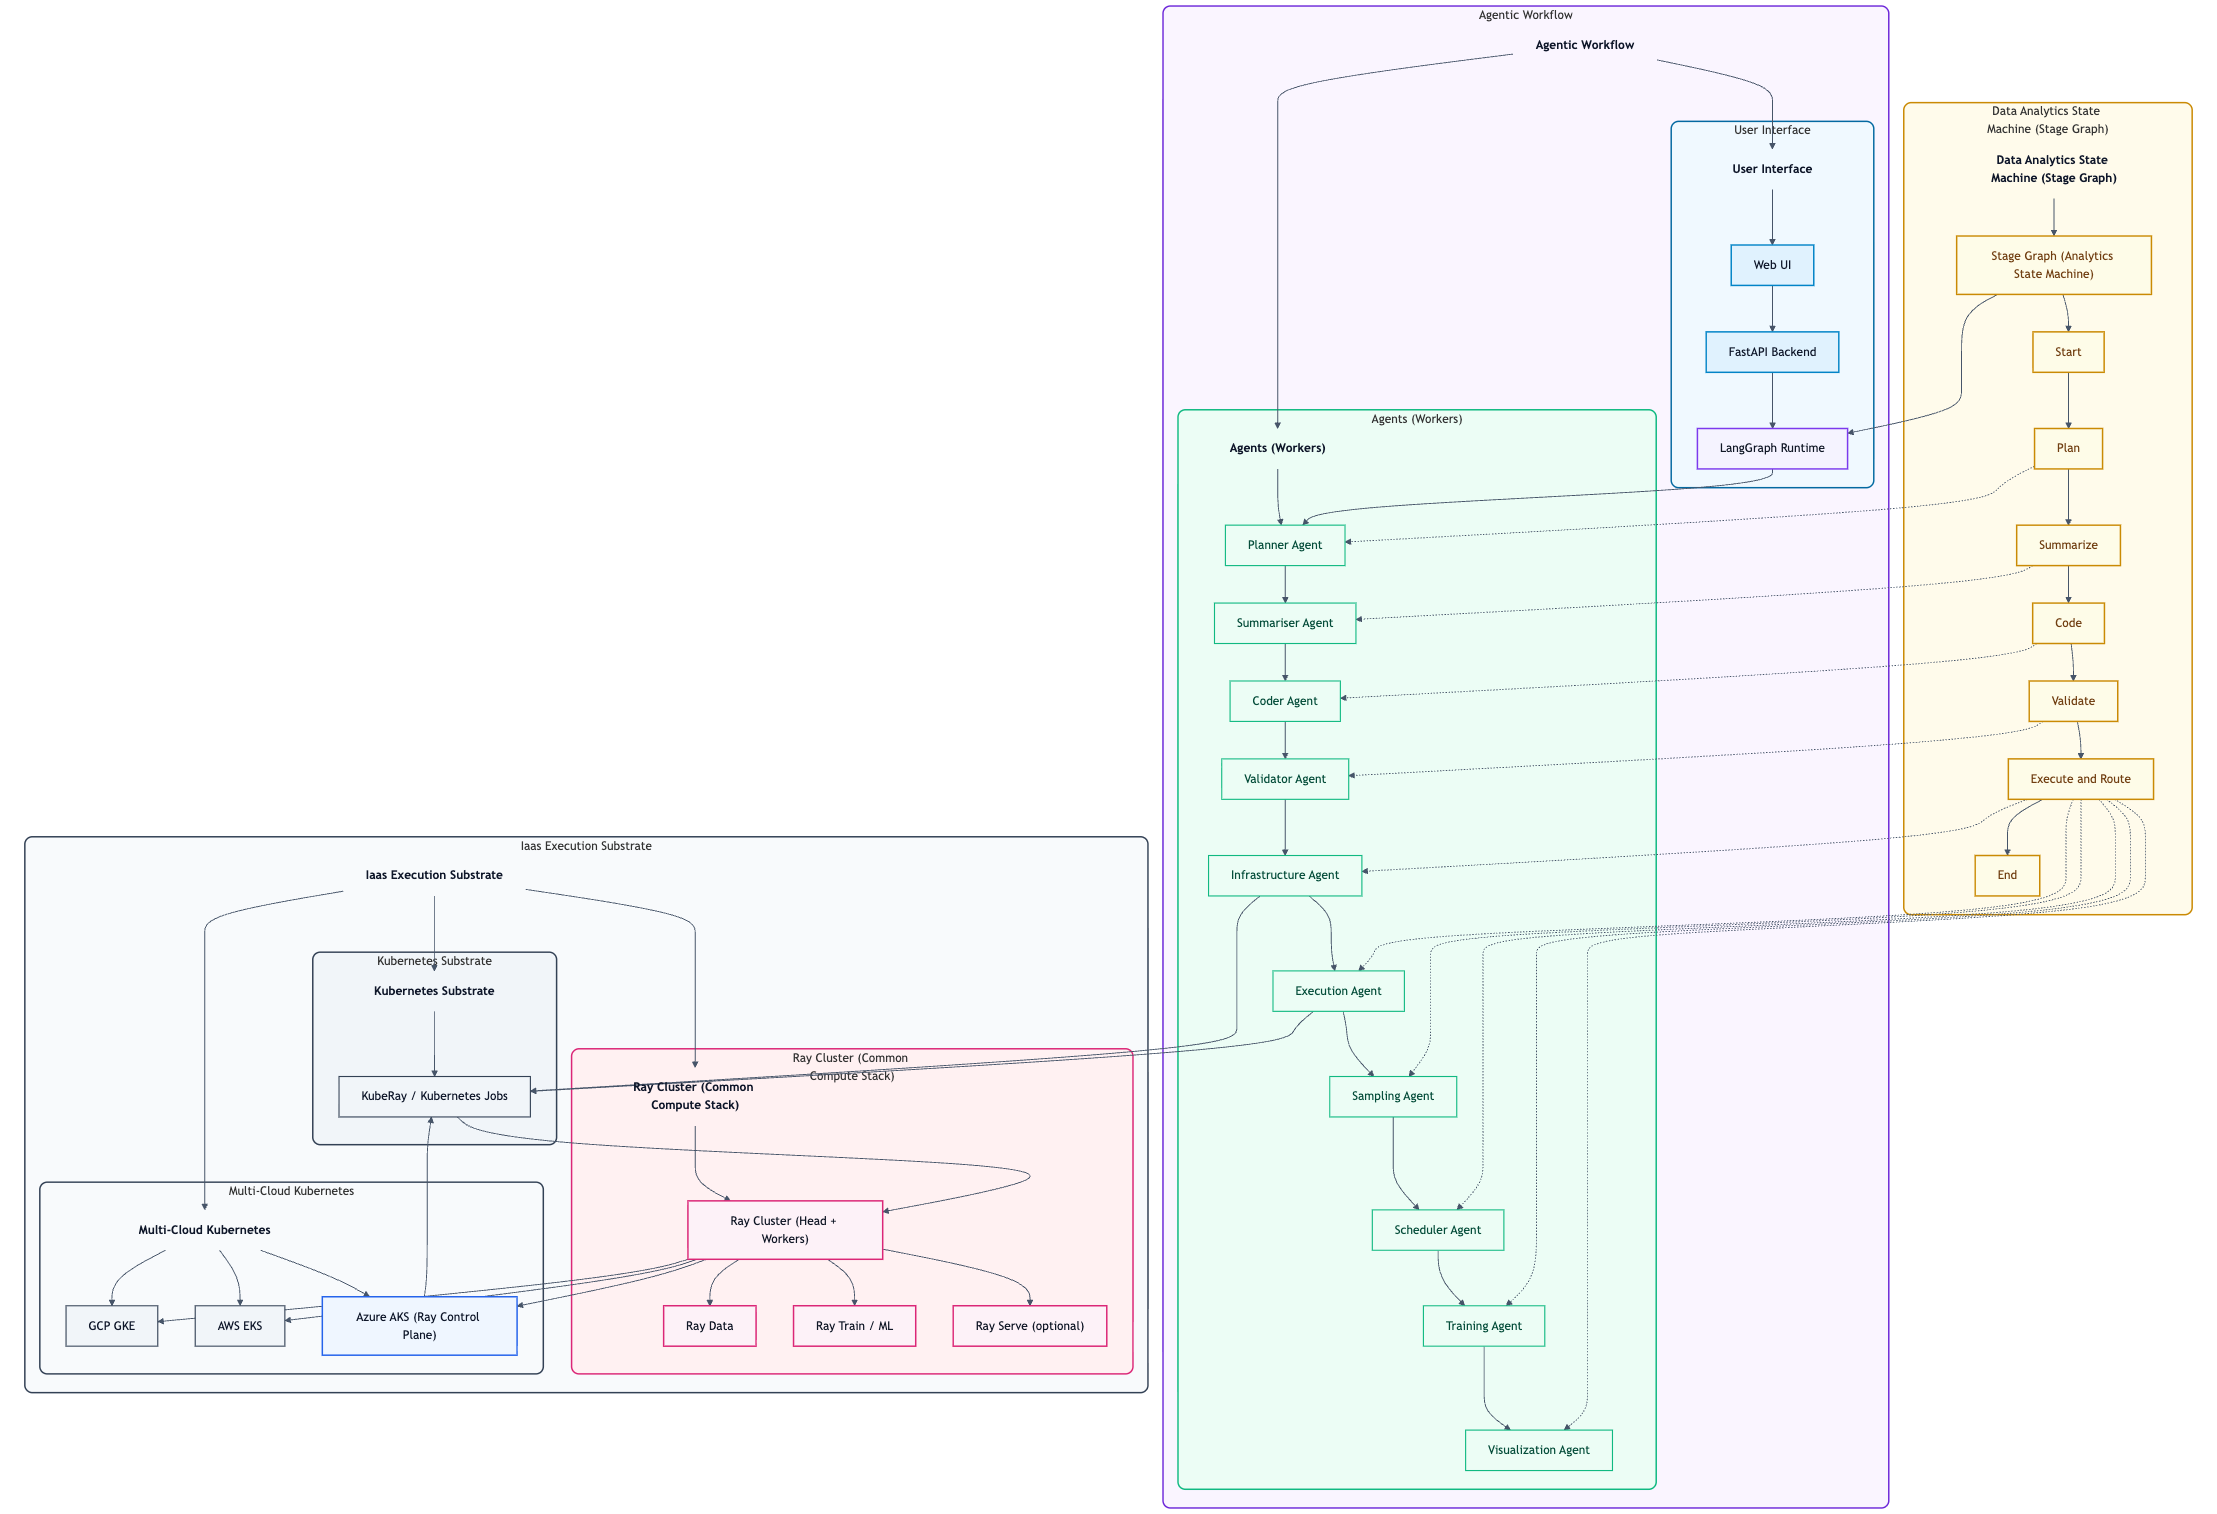
\includegraphics[width=\linewidth]{fig/Avaloka.png}
  \caption{Avaloka architecture showing the agentic workflow, optimizer-aware validation, MCP tool layer,
  and scalable execution substrate.}
  \label{fig:architecture}
\end{figure}

\paragraph{Decision-Making (Reasoning) Layer.}
Reasoning agents (Planner, Summariser, Coder, Validator) synthesize plans, draft code, and perform
cross-validations using samples and optimizer artifacts. No large-scale data mutation occurs at this stage.

\paragraph{Execution Layer.}
Once validated (and optionally user-reviewed), execution agents run ETL/analytics and model workflows on
scalable backends (e.g., Spark/Ray on Kubernetes), producing artifacts, metrics, and audit logs.

\paragraph{Graph-based transitions and shared state.}
LangGraph represents each agent as a node in a directed graph with explicit routing. A versioned typed
state object carries schemas, samples, contracts, plan diffs, and artifacts to avoid relying on long
chat histories.

\paragraph{Model Context Protocol (MCP) server.}
MCP servers act as standardized connectors to enterprise systems (databases, warehouses, catalogs, and
observability tools). Through MCP, agents retrieve schemas, statistics, provenance, and run safe read-only
inspections (e.g., \texttt{EXPLAIN}) before generating or executing transformations \citep{mcp_spec,mcp_servers}.

\paragraph{Core agents.}
\textbf{Planner} parses intent, selects a workflow, and defines acceptance criteria.
\textbf{Coder} produces pseudo-code and executable code grounded in schema previews and samples.
\textbf{Validator} performs syntax checks, static-semantic checks, and optimizer-aware plan validation.
\textbf{Executor} performs bounded dry runs on samples, then dispatches full runs to the execution substrate.

\paragraph{Execution substrate.}
Avaloka supports distributed execution (Ray/Kubernetes) and larger-than-memory processing (e.g., Daft-style
lazy transforms) for enterprise volumes \citep{ray,daft}. In the system, production jobs are deployed as
Kubernetes workloads to remain cloud-agnostic.

\paragraph{AutoML and inference endpoints.}
After producing a trainable dataset, Avaloka generates an AutoML training plan (feature set, splits,
baseline models, metrics), launches training jobs, tracks artifacts, and deploys an inference endpoint as
a production service. Statistical profiling and sampling are used to eliminate unnecessary feature work and
to select safe, effective training configurations early.

\section{Why ``Simple'' Insights and ML Still Take Too Long}
\label{sec:why_slow}
A recurring industry paradox is that even a seemingly simple question (e.g., ``weekly revenue by
segment'' or ``train a churn model'') can take days to weeks. The delay is not the query itself; it is
the prerequisite work to make data \emph{well-defined, stable, and safe} under real-world operational
constraints.

\paragraph{Semantic uncertainty and schema reality.}
Tables rarely encode meaning explicitly: primary keys are implicit, grain is undocumented, and
business entities are split across systems. Analysts spend time inferring join keys, resolving naming
ambiguity, handling nullable identifiers, and preventing fanout joins that silently duplicate facts.

\paragraph{Normalization and modeling defects.}
Normalization mistakes (or inconsistent dimensional modeling) force repeated ad-hoc fixes downstream:
duplicated attributes, denormalized snapshots without effective dates, mixed grains in one table, and
non-idempotent transformations. These defects are subtle and often only discovered after inconsistencies
appear in dashboards or model performance.

\paragraph{Formatting, storage layout, and performance tuning.}
Even for read-only analysis, performance depends on physical layout: partitioning, clustering/z-order,
indexes, column encoding, file sizes, and compaction. If the storage layout is misaligned with access
patterns, ``simple'' queries become expensive, slow, and unreliable under concurrency.

\paragraph{Data quality, bias, and leakage checks.}
Modeling requires more than clean rows: label correctness, missingness mechanisms, spurious correlations,
population shift, and leakage hazards must be identified. This work typically requires iterative
profiling, slicing, and sanity checks across segments and time windows.

\paragraph{Change management and pipeline reliability.}
Production datasets evolve. Schema drift, backfills, late-arriving data, and migration errors routinely
break jobs or (worse) introduce silent regressions. Hardening a dataset means adding contracts, tests,
rollbacks, and alerting, which is frequently the dominant time cost.

\paragraph{SRE constraints and governance overhead.}
Database SRE concerns (quotas, resource caps, noisy neighbors, stale statistics, plan regressions) and
governance requirements (access control, audit logging, provenance, PII handling) impose additional
steps before data can be safely used for analytics or ML.

\paragraph{How Avaloka addresses the bottleneck.}
Avaloka reduces the above latency by combining (i) robust sampling for fast distributional understanding,
(ii) self-inferential statistical profiling to propose constraints, grains, and candidate keys,
(iii) LLM+coding agents to generate transformations, tests, and training code, and (iv) optimizer-aware
validation gates (plan/cost/cardinality checks) before full execution. The result is a predictable path
from pointed-to data sources to trainable datasets and deployed inference endpoints, without requiring
data scientists to manually iterate through cleansing, feature-engineering rigmarole, and brittle
operational glue.

\section{Optimizer-Aware Robustness: From NL Intent to Safe Plans}
\label{sec:optimizer}
\paragraph{Why optimizers matter for agentic analytics.}
Enterprise robustness hinges on what actually executes: join orders, access paths, spill risk, and resource
consumption are governed by the database optimizer and its statistics. Avaloka treats optimizer artifacts
(\texttt{EXPLAIN} plans, estimated cardinalities, and cost deltas) as validation inputs, not debugging outputs.

\paragraph{Plan- and stats-grounded validation gates.}
Given candidate SQL or a transformation plan, the Validator enforces:
(i) syntactic validity; (ii) schema/type compatibility; (iii) plan sanity checks (e.g., cross joins, fanout
joins, missing predicates, unexpected full scans); and (iv) bounded trial execution on representative samples.
When available, lightweight metadata (table sizes, column stats/histograms) is used to detect selectivity
surprises that often trigger runaway queries.

\paragraph{Sampling-first exploration and approximate answers.}
Avaloka uses approximate sampling inspired by BlinkDB to quickly estimate selectivity and distributional
properties, then choose a sampling strategy to satisfy a latency or error target for exploration before
scaling execution \citep{blinkdb_dbdb}. Sampling also enables interactive approximate answers with explicit
error-time tradeoffs.

\paragraph{LLMs + coding agents + MCP tools.}
LLMs are used where they add leverage (candidate transformations, test generation, explanation synthesis),
while deterministic tools handle execution, plan inspection, and provenance logging. MCP standardizes access
to database estates and related tooling, allowing consistent audit controls across heterogeneous deployments.

\section{Agentic Workflow}
\label{sec:workflow}
The MVP workflow is implemented as a state machine with validation gates. The agent roster includes:
\begin{itemize}
  \item Planner: collects requirements and chooses the next action.
  \item Summariser: converts conversation into a structured job contract.
  \item Coder: generates pseudo-code and then executable code.
  \item Validator: performs syntax, static-semantic, and optimizer-aware checks.
  \item Executor: runs bounded sample jobs; dispatches full runs when safe.
  \item Scheduler: manages periodic runs and job operations.
  \item AutoML Trainer: generates training plans, runs training/inference, and deploys endpoints.
  \item Visualization: creates charts from outputs for fast insight.
\end{itemize}

Agents exchange a shared state object containing: dataset identifiers/showcases, schema snapshots, sampling
strategies, plan diffs, code artifacts, training configs, endpoint metadata, and audit logs. This enables
repeatability for scheduled jobs and supports rollback/retry without recomputation.

\section{Scheduling and Production Jobs}
\label{sec:scheduling}
Avaloka includes a Scheduler agent that creates production jobs and deploys them as Kubernetes workloads.
Users can request periodic jobs using cron-style parameters, retrieve task status, fetch prior results, or
cancel scheduled tasks. Scheduled runs reuse the validated workflow by passing serialized state into the
execution path, preserving the same validation gates at each run.

\section{AutoML Training, Efficient Feature Minimization, and Inference Endpoints}
\label{sec:training}
Avaloka's AutoML path targets an end-to-end outcome: a deployed inference endpoint backed by tracked
training artifacts.

\paragraph{Statistical profiling for feature minimization (design principle).}
Instead of manual feature engineering loops, Avaloka uses profiling signals (missingness, cardinality,
skewness, leakage risk, stability under sampling) to select a minimal feature set sufficient for a baseline
model. Candidate features are generated only when profiling indicates predictive gaps, reducing engineer time.

\paragraph{Training workflow.}
The AutoML Trainer agent:
(i) produces a training contract (target, splits, metrics, constraints);
(ii) generates training code with tests; (iii) runs small-sample pilots to validate data/label integrity;
(iv) scales training; and (v) registers a model and deploys an inference endpoint as a production service.
Experiment tracking and artifact management can be integrated with standard ML tracking stacks (e.g., MLflow).

\section{Operational Robustness and Failure Modes}
\label{sec:robustness}
We scope robustness to dominant real-world failure modes in data platforms:

\paragraph{Human data orchestration errors.}
Frequent failures include wrong join keys, wrong grain, silent duplication, and incorrect assumptions about
nullable keys. Avaloka mitigates these by generating explicit job contracts (inputs, join predicates, expected
row-count ranges) and running invariant checks on samples before full execution.

\paragraph{Schema validation and drift.}
Schema drift (renames, type changes, new enums) breaks pipelines and silently corrupts metrics. Avaloka
maintains schema context and validates transformations against it; scheduled jobs re-check compatibility at
runtime before launch.

\paragraph{Normalization and design defects.}
Normalization mistakes and inconsistent dimensional modeling cause ambiguous semantics and hard-to-fix logic.
Avaloka flags likely fanout joins and repeated/duplicated facts using schema relationships and plan signals.

\paragraph{Change management errors.}
Unsafe migrations and ad-hoc patches cause incidents. Avaloka treats database changes as first-class artifacts:
it generates migration plans, proposes backward-compatible sequences, gates execution on dry runs and plan diffs,
and provides rollback instructions.

\paragraph{Database SRE difficulties.}
SRE challenges include plan regressions, stale statistics, resource caps, and contention. Optimizer-aware
validation detects regressions early; sampling-first execution contains blast radius; Kubernetes deployment
simplifies policy enforcement and portability.

\paragraph{Cloud-agnostic deployment benefits.}
Executing the MVP exclusively on Kubernetes improves portability and repeatability across on-prem and multi-cloud
environments while keeping governance controls (secrets, policies, audit logs) consistent.

\section{Evaluation: Measuring Robustness and AutoML Productivity}
\label{sec:evaluation}
We evaluate Avaloka as an MVP on robustness outcomes and ML productivity rather than raw LLM accuracy.

\subsection{Benchmarks and tasks}
We align task design with multi-step data-agent benchmarks such as DABstep \citep{dabstep_adyen,dabstep_space}
and incorporate safety framing from AgenticData: An Agentic Data Analytics System for Heterogeneous Data\citep{agentswild2025,agentswild_site} to emphasize
prevention of irreversible production failures.

\subsection{Robustness metrics (primary)}
\begin{itemize}
  \item \textbf{Prevented execution failures / 100 tasks:} fraction of tasks where gates stop unsafe execution
  (invalid schema, fanout joins, cross joins, missing predicates, high-cost regressions).
  \item \textbf{Plan regression detection:} ability to detect large cost/cardinality deltas between candidate
  variants or between scheduled runs (pre/post drift).
  \item \textbf{Schema drift sensitivity:} detection rate under synthetic drift (rename, type widen, nullability
  changes, enum expansion) before execution.
  \item \textbf{Change safety score:} success rate of producing backward-compatible migration plans with rollback;
  failures include missing dependency ordering or unsafe operations.
  \item \textbf{Cost containment:} ratio of full-data executions avoided through sampling-first validation and
  preflight estimation.
\end{itemize}

\subsection{AutoML productivity metrics (reinforcing the design principle)}
\begin{itemize}
  \item \textbf{Time-to-trainable dataset:} time from request to a validated training dataset with schema/label checks.
  \item \textbf{Manual feature steps eliminated:} count of feature engineering steps avoided relative to a baseline
  manual workflow (measured as required human-authored transformations beyond the contract).
  \item \textbf{Time-to-endpoint:} time from request to a deployed inference endpoint with a registered model artifact.
\end{itemize}

\subsection{Experimental protocol}
We construct three suites:
(i) \emph{Exploration} tasks (aggregations, joins, window functions) with injected hazards;
(ii) \emph{Operations} tasks (migration planning, schema evolution) with drift;
(iii) \emph{SRE} tasks (plan regressions, stale stats, resource caps).
We compare:
(A) single-shot NL-to-SQL; (B) agentic verification without optimizer signals; (C) Avaloka with optimizer-aware
validation + sampling-first execution. For AutoML, we compare (D) a baseline manual feature pipeline against
(E) Avaloka's profiling-driven minimal-feature path.

\section{Limitations}
Avaloka assumes access to configured infrastructure (Kubernetes, database credentials, observability endpoints) for
advanced features. Long-running workflows require production-grade monitoring and incident response integrations.
Optimizer signals vary across databases; when unavailable, Avaloka falls back to conservative sampling-first checks.

\section{Conclusion}
Avaloka demonstrates how an optimizer-aware, sampling-first, agentic workflow can operationalize conversational
analytics and AutoML while retaining validation guarantees and cloud-agnostic deployment. The MVP evaluation focuses
on preventing operational errors and accelerating time-to-trainable dataset and time-to-endpoint, providing a practical
path from intent to production-grade jobs.

\begin{thebibliography}{99}

\bibitem[Song et~al.(2025)Song, Wang, Crispino, Jia, Montgomery, Potter, Siu, and Wang]{agentswild2025}
Dawn Song, Chenguang Wang, Nicholas Crispino, Ruoxi Jia, Kyle Montgomery, Yujin Potter,
Vincent Siu, and Zhun Wang.
\newblock \emph{AgenticData: An Agentic Data Analytics System for Heterogeneous Data}.
\newblock arXiv:2508.05002, 2025. \url{https://arxiv.org/abs/2508.05002}.

\bibitem[AgenticData: An Agentic Data Analytics System for Heterogeneous Data(2026)]{agentswild_site}
AgenticData: An Agentic Data Analytics System for Heterogeneous Data(ICLR 2026 Workshop).
\newblock \url{https://agentwild-workshop.github.io/}.

\bibitem[Egg et~al.(2025)Egg et~al.]{dabstep_adyen}
Alex Egg et al.
\newblock \emph{DABstep: Data Agent Benchmark for Multi-step Reasoning}.
\newblock arXiv:2506.23719, 2025. \url{https://arxiv.org/abs/2506.23719}.

\bibitem[Adyen and Hugging Face(2025)]{dabstep_space}
Adyen and Hugging Face.
\newblock \emph{DABstep Leaderboard (Hugging Face Space)}.
\newblock \url{https://huggingface.co/spaces/adyen/DABstep}.

\bibitem[DBDB(2025)]{blinkdb_dbdb}
Database of Databases.
\newblock \emph{BlinkDB}.
\newblock \url{https://dbdb.io/db/blinkdb}.

\bibitem[Ray(2025)]{ray}
Apache Ray documentation.
\newblock \url{https://docs.ray.io}.

\bibitem[Daft(2025)]{daft}
Daft documentation.
\newblock \url{https://www.getdaft.io}.

\bibitem[MCP(2025a)]{mcp_spec}
Model Context Protocol.
\newblock \emph{MCP Specification}.
\newblock \url{https://modelcontextprotocol.io/specification/}.

\bibitem[MCP(2025b)]{mcp_servers}
Model Context Protocol.
\newblock \emph{MCP Server Concepts}.
\newblock \url{https://modelcontextprotocol.io/docs/learn/server-concepts}.

\bibitem[Avaloka(2026)]{avaloka_site}
Avaloka.
\newblock \emph{Avaloka Product Website}.
\newblock \url{https://avaloka.ai}.

\end{thebibliography}

\end{document}
